\documentclass[11pt]{article}
\usepackage{amsmath, amssymb, physics, mathtools, bm}
\usepackage{tikz}
\usetikzlibrary{decorations.pathmorphing,arrows.meta,calc,positioning}
\usepackage[margin=2.3cm]{geometry}
\usepackage{siunitx, booktabs, hyperref}
\usepackage{braket}

\newcommand{\D}{\mathrm{D}}
\newcommand{\de}{\mathrm{d}}
\newcommand{\pd}[2]{\frac{\partial #1}{\partial #2}}
\newcommand{\pdd}[2]{\frac{\partial^{2} #1}{\partial #2^{2}}}
\newcommand{\Lap}{\nabla^{2}}
\newcommand{\fourvec}[1]{\underline{#1}}

\title{B2: Symmetry and Relativity\\ Model Solutions --- Trinity Term 2024}
\author{}
\date{}

\begin{document}
\maketitle

\noindent\textit{Conventions.} Metric $\eta_{\mu\nu}=\mathrm{diag}(+,-,-,-)$. $U^\mu=(\gamma c,\gamma\vb v)$, $U_\mu U^\mu=c^2$. $p^\mu=(E/c,\vb p)$, $p_\mu p^\mu=m^2c^2$. SI units; $c=\SI{2.998e8}{m\,s^{-1}}$, $M_e c^2=\SI{0.511}{MeV}$.

%==================================================================
\section*{Question 1 --- Photon--photon pair production, helicity, charge conjugation, and Compton/annihilation kinematics}

\textbf{Problem.} (a) Threshold $E_\gamma$ for $\gamma+\gamma_{\rm CMB}\to e^+e^-$ with $\varepsilon_{\rm CMB}=\SI{6.626e-4}{eV}$. (b) Boost flipping helicity of an electron $(M_e,p)$; massless case. (c) Show $\tau\to-\tau$ in the Lorentz force law gives $q\to-q$; rewrite the scalar $\mathcal{S}$ for a positron. (d) Compton: $\lambda_2-\lambda_1=(h/M_ec)(1-\cos\theta)$. (e) Two-photon annihilation: $\lambda_1+\lambda_2=(h/M_ec)(1-\cos\theta)$.

\subsection*{(a) Threshold for $\gamma+\gamma_{\rm CMB}\to e^+e^-$}

At threshold the pair is at rest in the CoM:
\[ s_{\min}=(2M_ec)^2=4M_e^2c^2. \]
Head-on geometry minimises $E_\gamma$:
\[ p_1^\mu=(E_\gamma/c)(1,1,0,0),\qquad p_2^\mu=(\varepsilon/c)(1,-1,0,0). \]
Compute the dot product with metric $(+,-,-,-)$:
\[ p_1\cdot p_2=\frac{E_\gamma}{c}\cdot\frac{\varepsilon}{c}-\frac{E_\gamma}{c}\cdot\left(-\frac{\varepsilon}{c}\right). \]
Combine the two terms:
\[ p_1\cdot p_2=\frac{2E_\gamma\varepsilon}{c^2}. \]
Form $s$ using $p_1^2=p_2^2=0$:
\[ s=(p_1+p_2)^2=2p_1\cdot p_2=\frac{4E_\gamma\varepsilon}{c^2}. \]
Equate to threshold $4M_e^2c^2$:
\[ \frac{4E_\gamma\varepsilon}{c^2}=4M_e^2c^2. \]
Solve for $E_\gamma$:
\[ E_\gamma^{\rm thr}=\frac{(M_ec^2)^2}{\varepsilon_{\rm CMB}}. \]
Insert numbers:
\[ E_\gamma^{\rm thr}=\frac{(\SI{5.11e5}{eV})^2}{\SI{6.626e-4}{eV}}. \]
Reduce:
\[ E_\gamma^{\rm thr}=\frac{\SI{2.611e11}{eV^2}}{\SI{6.626e-4}{eV}}=\SI{3.94e14}{eV}. \]
\begin{equation}
\boxed{\,E_\gamma^{\rm thr}=\frac{(M_ec^2)^2}{\varepsilon_{\rm CMB}}\approx\SI{3.9e14}{eV}\approx\SI{400}{TeV}.\,}
\end{equation}

\subsection*{(b) Helicity flip by boost}

Helicity $h=\hat{\vb s}\cdot\hat{\vb p}$. A collinear boost cannot rotate $\hat{\vb s}$, so flipping $h$ requires reversing $\vb p$. Boost along $+\hat{\vb p}$ at $\beta$:
\[ p_\parallel'=\gamma(p-\beta E/c). \]
Require $p_\parallel'<0$:
\[ p-\beta E/c<0. \]
Rearrange:
\[ \beta E/c>p. \]
Solve for $\beta$:
\[ \beta>\frac{pc}{E}. \]
Use the mass-shell $E=\sqrt{p^2c^2+M_e^2c^4}$ in the threshold value:
\begin{equation}
\boxed{\,\vec\beta=\frac{pc}{E}\hat{\vb p},\qquad E=\sqrt{p^2c^2+M_e^2c^4};\ \text{any larger }\beta\text{ along }+\hat{\vb p}\text{ flips helicity}.\,}
\end{equation}
Massless case: $E=pc$ requires $\beta=1$, not a Lorentz transformation. Hence helicity is Lorentz invariant for a photon and \emph{no frame} flips it.

\subsection*{(c) Charge conjugation via $\tau\to-\tau$ and the positron scalar}

Lorentz force law:
\begin{equation}
m\frac{\de^2 x^\alpha}{\de\tau^2}=qF^{\alpha\beta}U_\beta,\qquad U_\beta=\frac{\de x_\beta}{\de\tau}.
\label{eq:Q1c-lf}
\end{equation}
Under $\tau\to-\tau$ the second derivative is unchanged:
\[ \frac{\de^2 x^\alpha}{\de(-\tau)^2}=\frac{\de^2 x^\alpha}{\de\tau^2}. \]
The 4-velocity picks up a sign:
\[ U_\beta\to\frac{\de x_\beta}{\de(-\tau)}=-U_\beta. \]
Substitute into the force law:
\[ m\frac{\de^2 x^\alpha}{\de\tau^2}=qF^{\alpha\beta}(-U_\beta)=(-q)F^{\alpha\beta}U_\beta. \]
This is the equation for charge $-q$. $\tau$ is a Lorentz scalar, so the statement is frame-independent.

Stueckelberg--Feynman dictionary (positron $=$ time-reversed electron):
\[ p_2^i\to -p_{e^+}^f,\qquad p_2^f\to -p_{e^+}^i. \]
Substitute into each numerator bilinear:
\[ (p_2^f\cdot p_1^f)(p_1^i\cdot p_2^i)\to(-p_{e^+}^i\cdot p_1^f)(-p_1^i\cdot p_{e^+}^f)=(p_{e^+}^i\cdot p_1^f)(p_1^i\cdot p_{e^+}^f). \]
The second numerator term:
\[ (p_2^f\cdot p_2^i)(p_1^i\cdot p_1^f)\to\bigl((-p_{e^+}^i)\cdot(-p_{e^+}^f)\bigr)(p_1^i\cdot p_1^f). \]
Cancel the two minus signs:
\[ (p_2^f\cdot p_2^i)(p_1^i\cdot p_1^f)\to(p_{e^+}^i\cdot p_{e^+}^f)(p_1^i\cdot p_1^f). \]
The denominator:
\[ (p_2^f-p_1^i)^4\to(-p_{e^+}^i-p_1^i)^4=(p_{e^+}^i+p_1^i)^4. \]
Collect:
\begin{equation}
\boxed{\,\mathcal{S}_{ee^+}=\frac{(p_{e^+}^i\cdot p_1^f)(p_1^i\cdot p_{e^+}^f)+(p_{e^+}^i\cdot p_{e^+}^f)(p_1^i\cdot p_1^f)}{(p_{e^+}^i+p_1^i)^4}.\,}
\end{equation}
The denominator becomes the squared CoM energy $s=(p_{e^+}^i+p_1^i)^2$: $t$-channel M{\o}ller becomes $s$-channel Bhabha by crossing.

\subsection*{(d) Compton scattering}

4-momentum conservation:
\[ p_\gamma^i+p_e^i=p_\gamma^f+p_e^f. \]
Isolate the final electron:
\[ p_e^f=p_\gamma^i+p_e^i-p_\gamma^f. \]
Square both sides:
\[ (p_e^f)^2=(p_\gamma^i+p_e^i-p_\gamma^f)^2. \]
Expand the right-hand side:
\[ (p_e^f)^2=(p_\gamma^i)^2+(p_e^i)^2+(p_\gamma^f)^2+2p_\gamma^i\cdot p_e^i-2p_\gamma^f\cdot p_e^i-2p_\gamma^i\cdot p_\gamma^f. \]
Apply mass shells $(p_e^{i,f})^2=M_e^2c^2$, $(p_\gamma^{i,f})^2=0$:
\[ 0=2p_\gamma^i\cdot p_e^i-2p_\gamma^f\cdot p_e^i-2p_\gamma^i\cdot p_\gamma^f. \]
Divide by $2$:
\[ p_\gamma^i\cdot p_e^i-p_\gamma^f\cdot p_e^i=p_\gamma^i\cdot p_\gamma^f. \]
Evaluate the first dot product in lab frame ($p_e^i=(M_ec,\vec 0)$):
\[ p_\gamma^i\cdot p_e^i=(E_1/c)(M_ec)=M_eE_1. \]
Similarly for the second:
\[ p_\gamma^f\cdot p_e^i=(E_2/c)(M_ec)=M_eE_2. \]
Photon--photon dot product with $|\vec p_{1,2}|=E_{1,2}/c$ and opening angle $\theta$:
\[ p_\gamma^i\cdot p_\gamma^f=\frac{E_1E_2}{c^2}-\frac{E_1E_2}{c^2}\cos\theta. \]
Factor:
\[ p_\gamma^i\cdot p_\gamma^f=\frac{E_1E_2}{c^2}(1-\cos\theta). \]
Substitute all three into the divided equation:
\[ M_eE_1-M_eE_2=\frac{E_1E_2}{c^2}(1-\cos\theta). \]
Factor $M_e$:
\[ M_e(E_1-E_2)=\frac{E_1E_2}{c^2}(1-\cos\theta). \]
Divide by $M_eE_1E_2$:
\[ \frac{1}{E_2}-\frac{1}{E_1}=\frac{1-\cos\theta}{M_ec^2}. \]
Use $E=hc/\lambda$:
\[ \frac{\lambda_2}{hc}-\frac{\lambda_1}{hc}=\frac{1-\cos\theta}{M_ec^2}. \]
Multiply by $hc$:
\begin{equation}
\boxed{\,\lambda_2-\lambda_1=\frac{h}{M_ec}(1-\cos\theta).\,}
\label{eq:Q1d-compton}
\end{equation}
Since $1-\cos\theta\geq 0$, $\lambda_2\geq\lambda_1$: the \emph{incident} photon (1) is shorter.

\subsection*{(e) Two-photon annihilation}

Process $e^-(p_e)+e^+(p_{e^+})\to\gamma_1(k_1)+\gamma_2(k_2)$, positron at rest. Conservation:
\[ p_e+p_{e^+}=k_1+k_2. \]
Isolate the electron:
\[ p_e=k_1+k_2-p_{e^+}. \]
Square both sides:
\[ p_e^2=(k_1+k_2-p_{e^+})^2. \]
Expand the right-hand side:
\[ p_e^2=k_1^2+k_2^2+p_{e^+}^2+2k_1\cdot k_2-2k_1\cdot p_{e^+}-2k_2\cdot p_{e^+}. \]
Apply mass shells $p_e^2=p_{e^+}^2=M_e^2c^2$, $k_1^2=k_2^2=0$:
\[ 0=2k_1\cdot k_2-2k_1\cdot p_{e^+}-2k_2\cdot p_{e^+}. \]
Divide by $2$ and rearrange:
\[ k_1\cdot k_2=k_1\cdot p_{e^+}+k_2\cdot p_{e^+}. \]
Evaluate dot products in positron rest frame ($p_{e^+}=(M_ec,\vec 0)$):
\[ k_i\cdot p_{e^+}=(E_i/c)(M_ec)=M_eE_i. \]
Photon--photon dot product with opening angle $\theta$:
\[ k_1\cdot k_2=\frac{E_1E_2}{c^2}-\frac{E_1E_2}{c^2}\cos\theta=\frac{E_1E_2}{c^2}(1-\cos\theta). \]
Substitute into the rearranged conservation equation:
\[ \frac{E_1E_2}{c^2}(1-\cos\theta)=M_eE_1+M_eE_2. \]
Factor $M_e$ on the right:
\[ \frac{E_1E_2}{c^2}(1-\cos\theta)=M_e(E_1+E_2). \]
Divide by $M_eE_1E_2$:
\[ \frac{1-\cos\theta}{M_ec^2}=\frac{1}{E_1}+\frac{1}{E_2}. \]
Substitute $E_i=hc/\lambda_i$:
\[ \frac{1-\cos\theta}{M_ec^2}=\frac{\lambda_1}{hc}+\frac{\lambda_2}{hc}. \]
Multiply by $hc$:
\begin{equation}
\boxed{\,\lambda_1+\lambda_2=\frac{h}{M_ec}(1-\cos\theta).\,}
\end{equation}
Sign change vs.\ \eqref{eq:Q1d-compton} reflects the crossing $k\to-k$. At $\theta=\pi$ with $\vec p_e=\vec 0$: $\lambda_1=\lambda_2=h/(M_ec)$, two back-to-back \SI{511}{keV} gammas.

%==================================================================
\section*{Question 2 --- Charged-particle motion in $F^{\mu\nu}$, gauge invariance, plane waves and field invariants}

\textbf{Problem.} (a) Pure $\vec B$: show $\vec F\perp\vec v$ and find Larmor radius. (b) From $\partial_\nu\partial^\nu A^\mu-\partial^\mu\partial_\nu A^\nu=-\mu_0 J^\mu$ with static $A^0$ and $\vec A=0$, recover Poisson and identify $J^\mu$. (c) Plane wave $A^\mu=\epsilon^\mu\sin(k\cdot x)$: derive $F^{0i},F^{ij}$ and source-free condition. (d) Dual tensor and invariants; show $\vec E\perp\vec B$, $|\vec B|=|\vec E|/c$ gauge-free. (e) Find $B_1,B_2$ from invariants.

\subsection*{(a) Pure magnetic field}

Covariant equation:
\begin{equation}
m\,\frac{\de U^\alpha}{\de\tau}=qF^{\alpha\beta}U_\beta.
\end{equation}
With $\vec E=0$ only the spatial components of $F^{\alpha\beta}$ survive. Take $\alpha=0$:
\[ m\,\frac{\de(\gamma c)}{\de\tau}=qF^{0\beta}U_\beta=0. \]
Hence $\gamma$ and $|\vec v|$ are constant. Spatial component, using $\de/\de\tau=\gamma\,\de/\de t$:
\[ \frac{\de(\gamma m\vec v)}{\de t}=q\,\vec v\times\vec B. \]
Since $\gamma$ is constant the 3-force is:
\[ \vec F=\gamma m\frac{\de\vec v}{\de t}=q\,\vec v\times\vec B. \]
Dot with $\vec v$:
\[ \vec v\cdot\vec F=q\,\vec v\cdot(\vec v\times\vec B)=0. \]
So $\vec F\perp\vec v$. Take $\vec v\perp\vec B$ so the trajectory lies in a plane; force magnitude:
\[ |\vec F|=|q|\,vB. \]
Equate to centripetal $|\vec F|=\gamma m v^2/r$ (valid because $\gamma$ is constant):
\[ \frac{\gamma mv^2}{r}=qvB. \]
Cancel one factor of $v$:
\[ \frac{\gamma mv}{r}=qB. \]
Solve for $r$:
\begin{equation}
\boxed{\,r=\frac{\gamma mv}{qB}=\frac{p}{qB}.\,}
\end{equation}
Assumptions: (i) $\vec E=0$; (ii) $\vec v\perp\vec B$ (otherwise a helix of the same radius); (iii) $\gamma$ constant.

\subsection*{(b) Recovering Poisson}

\begin{equation}
\partial_\nu\partial^\nu A^\mu-\partial^\mu(\partial_\nu A^\nu)=-\mu_0 J^\mu.
\label{eq:Q2b-wave}
\end{equation}
Set $\vec A=0$ and $A^0=A^0(\vec x)$ (time-independent). The gauge term:
\[ \partial_\nu A^\nu=\partial_0 A^0+\partial_i A^i=0+0=0. \]
Take $\mu=0$. Static $A^0$ removes the time derivative from $\partial_\nu\partial^\nu$:
\[ \partial_\nu\partial^\nu A^0=\nabla^2 A^0. \]
Substitute into \eqref{eq:Q2b-wave} with $J^0=c\rho$ and the gauge term vanishing:
\[ \nabla^2 A^0=-\mu_0 c\rho. \]
Use $A^0=\phi/c$:
\[ \frac{1}{c}\nabla^2\phi=-\mu_0 c\rho. \]
Multiply through by $c$:
\[ \nabla^2\phi=-\mu_0 c^2\rho. \]
Use $\mu_0 c^2=1/\varepsilon_0$:
\begin{equation}
\boxed{\,\nabla^2\phi=-\frac{\rho}{\varepsilon_0}.\,}
\end{equation}
Take $\mu=i$ in \eqref{eq:Q2b-wave}. With $\vec A=0$ and $\partial_\nu A^\nu=0$:
\[ 0-0=-\mu_0 J^i. \]
Solve:
\[ J^i=0. \]
Hence
\begin{equation}
\boxed{\,J^\mu=(c\rho,\vec 0).\,}
\end{equation}
No gauge was fixed: time-independence of $A^0$ alone killed the gauge term.

\subsection*{(c) Plane-wave field tensor}

Differentiate $A^\mu=\epsilon^\mu\sin(k\cdot x)$:
\[ \partial^\mu A^\nu=\epsilon^\nu k^\mu\cos(k\cdot x). \]
Form the field tensor:
\begin{equation}
F^{\mu\nu}=\partial^\mu A^\nu-\partial^\nu A^\mu=(k^\mu\epsilon^\nu-k^\nu\epsilon^\mu)\cos(k\cdot x).
\label{eq:Q2c-Fmunu}
\end{equation}
Compute $F^{0i}$ with $\partial^0=\partial_0=(1/c)\partial_t$ and $\partial^i=-\partial_i$:
\[ F^{0i}=\partial^0 A^i-\partial^i A^0=\frac{1}{c}\partial_t A^i+\partial_i(\phi/c). \]
Factor $1/c$:
\[ F^{0i}=\frac{1}{c}\left(\partial_t A^i+\partial_i\phi\right). \]
Use $E^i=-\partial_t A^i-\partial_i\phi$:
\[ F^{0i}=-\frac{E^i}{c}. \]
For the spatial--spatial block use $\vec B=\nabla\times\vec A$, so $(\nabla\times\vec A)^k=\varepsilon^{kij}\partial_i A^j$:
\[ \partial_i A^j-\partial_j A^i=\varepsilon^{ijk}B_k. \]
Identify with $F^{ij}=\partial^i A^j-\partial^j A^i$ (sign convention of the problem):
\begin{equation}
\boxed{\,F^{0i}=-\frac{E^i}{c},\qquad F^{ij}=\varepsilon^{ijk}B_k.\,}
\end{equation}
Source-free Maxwell: $\partial_\mu F^{\mu\nu}=0$. Differentiate \eqref{eq:Q2c-Fmunu}:
\[ \partial_\mu F^{\mu\nu}=-(k_\mu k^\mu\epsilon^\nu-k^\nu k_\mu\epsilon^\mu)\sin(k\cdot x). \]
Collect:
\[ \partial_\mu F^{\mu\nu}=-[k^2\epsilon^\nu-k^\nu(k\cdot\epsilon)]\sin(k\cdot x). \]
Vanishing for all $\nu$ requires
\[ k^2=0\quad\text{and}\quad k\cdot\epsilon=0. \]
The first is the lightlike dispersion; the second is forced transversality (not a gauge choice). The trivial $\epsilon^\nu\propto k^\nu$ is pure gauge with $F^{\mu\nu}=0$.

\subsection*{(d) Dual tensor, invariants, $\vec E\perp\vec B$}

Definition:
\[ \tilde F^{\mu\nu}=\tfrac12\varepsilon^{\mu\nu\alpha\beta}F_{\alpha\beta}. \]
Component computation (with $\varepsilon_{0123}=+1$, so $\varepsilon^{0123}=-1$ in metric $(+,-,-,-)$):
\begin{equation}
\tilde F^{\mu\nu}=\begin{pmatrix}0&-B_x&-B_y&-B_z\\B_x&0&E_z/c&-E_y/c\\B_y&-E_z/c&0&E_x/c\\B_z&E_y/c&-E_x/c&0\end{pmatrix}.
\end{equation}
Two field invariants:
\[ F_{\mu\nu}F^{\mu\nu}=2\!\left(\vec B^2-\vec E^2/c^2\right),\qquad F_{\mu\nu}\tilde F^{\mu\nu}\propto\vec E\cdot\vec B. \]
Apply \eqref{eq:Q2c-Fmunu} to compute the first invariant:
\[ F^{\mu\nu}F_{\mu\nu}=(k^\mu\epsilon^\nu-k^\nu\epsilon^\mu)(k_\mu\epsilon_\nu-k_\nu\epsilon_\mu)\cos^2(k\cdot x). \]
Expand the product term by term:
\[ F^{\mu\nu}F_{\mu\nu}=\bigl[(k\!\cdot\!k)(\epsilon\!\cdot\!\epsilon)-(k\!\cdot\!\epsilon)^2-(k\!\cdot\!\epsilon)^2+(k\!\cdot\!k)(\epsilon\!\cdot\!\epsilon)\bigr]\cos^2(k\cdot x). \]
Combine like terms:
\[ F_{\mu\nu}F^{\mu\nu}=2\bigl[k^2\epsilon^2-(k\cdot\epsilon)^2\bigr]\cos^2(k\cdot x). \]
Compute the dual contraction:
\[ \varepsilon_{\mu\nu\alpha\beta}F^{\mu\nu}F^{\alpha\beta}\propto\varepsilon_{\mu\nu\alpha\beta}(k^\mu\epsilon^\nu-k^\nu\epsilon^\mu)(k^\alpha\epsilon^\beta-k^\beta\epsilon^\alpha). \]
Each term has two $k$'s and two $\epsilon$'s contracted with the totally antisymmetric tensor:
\[ \varepsilon_{\mu\nu\alpha\beta}k^\mu k^\alpha=0,\qquad\varepsilon_{\mu\nu\alpha\beta}\epsilon^\nu\epsilon^\beta=0. \]
Hence
\[ F_{\mu\nu}\tilde F^{\mu\nu}=0\Rightarrow\vec E\cdot\vec B=0. \]
\begin{equation}
\boxed{\,\vec E\cdot\vec B=0\,}\qquad\text{(gauge-free).}
\end{equation}
Apply $k^2=0$, $k\cdot\epsilon=0$ from (c) to the first invariant:
\[ F_{\mu\nu}F^{\mu\nu}=2[0-0]\cos^2(k\cdot x)=0. \]
Equate to $2(\vec B^2-\vec E^2/c^2)$:
\[ \vec B^2-\vec E^2/c^2=0. \]
Solve:
\begin{equation}
\boxed{\,|\vec B|=\frac{|\vec E|}{c}.\,}
\end{equation}
Both invariants vanish: a free plane wave is a null EM field.

\subsection*{(e) Finding $B_1,B_2$}

Two invariants (from (d)): $\vec E\cdot\vec B$ and $|\vec E|^2-c^2|\vec B|^2$.
Frame $S$: $\vec E=(E,E,0)$, $\vec B=(0,0,2E/c)$.
Compute the first invariant in $S$:
\[ \vec E\cdot\vec B=E\cdot 0+E\cdot 0+0\cdot(2E/c)=0. \]
Compute the second invariant in $S$:
\[ |\vec E|^2-c^2|\vec B|^2=(E^2+E^2)-c^2\cdot(2E/c)^2=2E^2-4E^2=-2E^2. \]
Frame $S'$: $\vec E\,'=(0,0,E)$, $\vec B\,'=(B_1,E/c,B_2)$.
Compute the first invariant in $S'$:
\[ \vec E\,'\cdot\vec B\,'=0\cdot B_1+0\cdot(E/c)+E\cdot B_2=EB_2. \]
Equate to $S$:
\[ EB_2=0\Rightarrow\boxed{\,B_2=0.\,} \]
Compute the second invariant in $S'$ (with $B_2=0$):
\[ |\vec E\,'|^2-c^2|\vec B\,'|^2=E^2-c^2(B_1^2+E^2/c^2). \]
Expand:
\[ |\vec E\,'|^2-c^2|\vec B\,'|^2=E^2-c^2B_1^2-E^2=-c^2B_1^2. \]
Equate to $S$:
\[ -c^2 B_1^2=-2E^2. \]
Divide by $-c^2$:
\[ B_1^2=\frac{2E^2}{c^2}. \]
Take square root:
\begin{equation}
\boxed{\,B_1=\pm\frac{\sqrt{2}\,E}{c}.\,}
\end{equation}
Sign ambiguity: the invariants do not fix the boost orientation.

%==================================================================
\section*{Question 3 --- Length contraction, the wavefront invariant, beaming and aberration}

\textbf{Problem.} (a) 3--4--5 triangle in $S'$ with $3L$ along $\hat{\vb x}'$, $S'$ boosted at $v$: find sides in $S$, area in $S'$, hypotenuse angle in $S$. (b) Show $L^2$ between two points on a wavefront is Lorentz invariant. (c) Show $I'/I=(\omega'/\omega)^2$. (d) Aberration formula and $\de\Omega/\de\Omega'=(\omega'/\omega)^2$. (e) Combine: $(\de P/\de\Omega')/(\de P/\de\Omega)=(\omega'/\omega)^4$.

\subsection*{(a) The 3--4--5 triangle in $S$}

Length contraction acts only along $\hat{\vb x}$. The shortest side ($3L$) lies along $\hat{\vb x}'$:
\[ 3L\to 3L/\gamma. \]
The medium side ($4L$) lies perpendicular to the boost (along $\hat{\vb y}'$):
\[ 4L\to 4L. \]
The hypotenuse runs in $S$ from $(3L/\gamma,0)$ to $(0,4L)$. Apply Pythagoras:
\[ \text{hypotenuse}^2=(3L/\gamma)^2+(4L)^2. \]
Take the square root:
\[ \text{hypotenuse}=L\sqrt{9/\gamma^2+16}. \]
Area in $S'$ (proper frame):
\[ A'=\tfrac12\cdot 3L\cdot 4L=6L^2. \]
Angle of hypotenuse with $x$-axis in $S$ (acute):
\[ \tan\alpha_S=\frac{4L}{3L/\gamma}=\frac{4\gamma}{3}. \]
\begin{equation}
\boxed{\,3L\to\frac{3L}{\gamma},\ 4L\to 4L,\ 5L\to L\sqrt{16+9/\gamma^2},\ A'=6L^2,\ \tan\alpha_S=\frac{4\gamma}{3}.\,}
\end{equation}
Limit $v\to c$: $\gamma\to\infty$, triangle collapses to a segment of length $4L$ along $\hat{\vb y}$.

\subsection*{(b) Wavefront distance invariance}

Phase $\Phi=\omega t-\vec k\cdot\vec x$. Take two points $A,B$ on the same wavefront in $S$ at $t=0$. Place $A$ at origin:
\[ A:(0,\vec 0),\qquad B:(0,\vec r). \]
Wavefront geometry requires $\vec r\perp\hat{\vb k}$ (B on same constant-phase surface as A):
\[ L^2=|\vec r|^2=r_x^2+r_y^2+r_z^2. \]
Boost along $+\hat{\vb x}$ to $S'$ and apply the Lorentz transformation to event $B$:
\[ c\Delta t'=\gamma(c\cdot 0-\beta r_x)=-\gamma\beta r_x. \]
Spatial coordinates of $B$ in $S'$:
\[ \Delta x'=\gamma(r_x-\beta\cdot 0)=\gamma r_x,\qquad \Delta y'=r_y,\qquad \Delta z'=r_z. \]
In $S'$, events $A$ and $B$ are not simultaneous, so direct subtraction does not give the wavefront distance. Use the invariant interval $\Delta s^2=c^2\Delta t^2-|\Delta\vec r|^2$. In $S$:
\[ \Delta s^2=0-L^2=-L^2. \]
Compute $\Delta s^2$ in $S'$ from the boosted coordinates:
\[ \Delta s^2=c^2\Delta t'^2-(\Delta x'^2+\Delta y'^2+\Delta z'^2). \]
Substitute the boost results:
\[ \Delta s^2=\gamma^2\beta^2 r_x^2-\gamma^2 r_x^2-r_y^2-r_z^2. \]
Factor the $r_x^2$ pieces:
\[ \Delta s^2=\gamma^2(\beta^2-1)r_x^2-r_y^2-r_z^2. \]
Use $\gamma^2(\beta^2-1)=-1$:
\[ \Delta s^2=-r_x^2-r_y^2-r_z^2=-L^2. \]
Slide $B$ along the null wavefront in $S'$ to common $t'=0$; this does not change $\Delta s^2$. At common $t'=0$ the interval becomes $\Delta s^2=-L'^2$:
\begin{equation}
\boxed{\,L'^2=r_x^2+r_y^2+r_z^2=L^2.\,}
\end{equation}
The wavefront-intrinsic distance is the projection onto a null hypersurface and is preserved by Lorentz transformations.

\subsection*{(c) Intensity ratio}

Define a flux box of wavefront area $A$ and length $\lambda$, containing photon number density $n$. Intensity (energy per area per time):
\[ I=n\hbar\omega\,c. \]
Total photons in the box, $nV=nA\lambda$, is Lorentz invariant:
\[ nA\lambda=n'A'\lambda'. \]
Wavefront area is invariant by (b): $A=A'$:
\[ n\lambda=n'\lambda'. \]
Solve for density ratio:
\[ \frac{n'}{n}=\frac{\lambda}{\lambda'}=\frac{\omega'}{\omega}. \]
Form the intensity ratio:
\[ \frac{I'}{I}=\frac{n'\hbar\omega' c}{n\hbar\omega c}=\frac{n'}{n}\cdot\frac{\omega'}{\omega}. \]
Substitute:
\[ \frac{I'}{I}=\frac{\omega'}{\omega}\cdot\frac{\omega'}{\omega}. \]
\begin{equation}
\boxed{\,\frac{I'}{I}=\left(\frac{\omega'}{\omega}\right)^{\!2}.\,}
\end{equation}

\subsection*{(d) Aberration and solid-angle ratio}

Doppler (given):
\begin{equation}
\omega=\gamma\omega'(1-\beta\cos\theta').
\label{eq:Q3d-doppler}
\end{equation}
Inverse Doppler (source frame to observer, observer moves at $-\beta$ in source frame):
\[ \omega'=\gamma\omega(1+\beta\cos\theta). \]
Multiply the two relations:
\[ \omega\omega'=\gamma^2\omega\omega'(1-\beta\cos\theta')(1+\beta\cos\theta). \]
Divide by $\omega\omega'$:
\[ 1=\gamma^2(1-\beta\cos\theta')(1+\beta\cos\theta). \]
Solve for $(1+\beta\cos\theta)$:
\[ 1+\beta\cos\theta=\frac{1}{\gamma^2(1-\beta\cos\theta')}. \]
Subtract $1$:
\[ \beta\cos\theta=\frac{1}{\gamma^2(1-\beta\cos\theta')}-1. \]
Common denominator:
\[ \beta\cos\theta=\frac{1-\gamma^2(1-\beta\cos\theta')}{\gamma^2(1-\beta\cos\theta')}. \]
Expand the numerator:
\[ \text{numerator}=1-\gamma^2+\gamma^2\beta\cos\theta'. \]
Use $1-\gamma^2=-\gamma^2\beta^2$:
\[ \text{numerator}=-\gamma^2\beta^2+\gamma^2\beta\cos\theta'=\gamma^2\beta(\cos\theta'-\beta). \]
Substitute and cancel $\gamma^2$:
\[ \beta\cos\theta=\frac{\beta(\cos\theta'-\beta)}{1-\beta\cos\theta'}. \]
Cancel $\beta$:
\begin{equation}
\boxed{\,\cos\theta=\frac{\cos\theta'-\beta}{1-\beta\cos\theta'}.\,}
\end{equation}
Differentiate with respect to $\cos\theta'$:
\[ \frac{\de(\cos\theta)}{\de(\cos\theta')}=\frac{(1-\beta\cos\theta')-(\cos\theta'-\beta)(-\beta)}{(1-\beta\cos\theta')^2}. \]
Expand numerator:
\[ \text{numerator}=1-\beta\cos\theta'+\beta\cos\theta'-\beta^2=1-\beta^2. \]
Substitute:
\[ \frac{\de(\cos\theta)}{\de(\cos\theta')}=\frac{1-\beta^2}{(1-\beta\cos\theta')^2}=\frac{1}{\gamma^2(1-\beta\cos\theta')^2}. \]
Use $\de\Omega=-\de(\cos\theta)\,\de\varphi$, $\de\varphi=\de\varphi'$:
\[ \frac{\de\Omega}{\de\Omega'}=\frac{1}{\gamma^2(1-\beta\cos\theta')^2}. \]
Identify $\gamma(1-\beta\cos\theta')=\omega/\omega'$ from \eqref{eq:Q3d-doppler}:
\begin{equation}
\boxed{\,\frac{\de\Omega}{\de\Omega'}=\left(\frac{\omega'}{\omega}\right)^{\!2}.\,}
\end{equation}

\subsection*{(e) Fourth-power beaming}

At the source, a wavefront patch of (invariant) area $\de A$ carries power $\de P=I\,\de A$ into solid angle $\de\Omega$. The same patch is seen at $\de\Omega'$ in the observer frame:
\[ \frac{\de P}{\de\Omega}=\frac{I\,\de A}{\de\Omega},\qquad\frac{\de P}{\de\Omega'}=\frac{I'\,\de A}{\de\Omega'}. \]
Form the ratio:
\[ \frac{\de P/\de\Omega'}{\de P/\de\Omega}=\frac{I'}{I}\cdot\frac{\de\Omega}{\de\Omega'}. \]
Substitute (c) $I'/I=(\omega'/\omega)^2$ and (d) $\de\Omega/\de\Omega'=(\omega'/\omega)^2$:
\[ \frac{\de P/\de\Omega'}{\de P/\de\Omega}=\left(\frac{\omega'}{\omega}\right)^{\!2}\cdot\left(\frac{\omega'}{\omega}\right)^{\!2}. \]
Combine:
\begin{equation}
\boxed{\,\frac{\de P/\de\Omega'}{\de P/\de\Omega}=\left(\frac{\omega'}{\omega}\right)^{\!4}.\,}
\end{equation}

%==================================================================
\section*{Question 4 --- Constant proper acceleration and the Rindler horizon}

\textbf{Problem.} (a) Constant 3-force $F_0$ from rest: find $v(t),x(t)$ and Newtonian limit. (b) Worldline $x^2-c^2t^2=c^4/a_0^2$: show $a_0$ is the proper acceleration. (c) Rewrite via $\sinh\omega=a_0t/c$ in terms of proper time. (d) Photon from $(t,x)=(-D/c,0)$: find $\tau_{\rm meet}$. (e) Show photons emitted at $t>0$ never catch up; sketch.

\subsection*{(a) Velocity and displacement}

Integrate $\de p/\de t=F_0$ from rest:
\[ p(t)=F_0 t. \]
Use $p=\gamma mv=mv/\sqrt{1-v^2/c^2}$ and square:
\[ p^2(1-v^2/c^2)=m^2v^2. \]
Expand:
\[ p^2=m^2v^2+p^2v^2/c^2. \]
Factor $v^2$ on the right:
\[ p^2=v^2(m^2+p^2/c^2). \]
Solve for $v$:
\[ v=\frac{pc}{\sqrt{p^2+m^2c^2}}. \]
Substitute $p=F_0t$ and rearrange to the form requested:
\begin{equation}
\boxed{\,v(t)=\frac{F_0t/m}{\sqrt{1+F_0^2t^2/(m^2c^2)}}.\,}
\end{equation}
Integrate $x(t)=\int_0^t v\,\de t'$ with substitution $u=1+F_0^2 t'^2/(m^2c^2)$, $\de u=2F_0^2 t'/(m^2c^2)\,\de t'$:
\begin{equation}
\boxed{\,x(t)=\frac{mc^2}{F_0}\!\left(\sqrt{1+\frac{F_0^2t^2}{m^2c^2}}-1\right).\,}
\end{equation}
Non-relativistic limit $F_0t\ll mc$, expand $\sqrt{1+\epsilon}\approx 1+\epsilon/2$:
\[ x(t)\approx\frac{mc^2}{F_0}\!\left(1+\frac{F_0^2t^2}{2m^2c^2}-1\right). \]
Cancel and simplify:
\[ x(t)\approx\frac{F_0t^2}{2m}. \]

\subsection*{(b) Identifying $a_0$ as proper acceleration}

Parametrise the hyperbola:
\[ x=\frac{c^2}{a_0}\cosh\eta,\qquad ct=\frac{c^2}{a_0}\sinh\eta. \]
Differentiate:
\[ \frac{\de x}{\de\eta}=\frac{c^2}{a_0}\sinh\eta,\qquad\frac{\de(ct)}{\de\eta}=\frac{c^2}{a_0}\cosh\eta. \]
Compute the proper-time line element from $\de s^2=c^2\de t^2-\de x^2$:
\[ \left(c\frac{\de t}{\de\eta}\right)^{\!2}-\left(\frac{\de x}{\de\eta}\right)^{\!2}=\frac{c^4}{a_0^2}(\cosh^2\eta-\sinh^2\eta)=\frac{c^4}{a_0^2}. \]
Equate with $c^2(\de\tau/\de\eta)^2$:
\[ c^2\left(\frac{\de\tau}{\de\eta}\right)^{\!2}=\frac{c^4}{a_0^2}. \]
Solve and integrate:
\[ \frac{\de\tau}{\de\eta}=\frac{c}{a_0}\ \Rightarrow\ \eta=\frac{a_0\tau}{c}. \]
4-velocity $U^\mu=\de x^\mu/\de\tau$, with $\de/\de\tau=(a_0/c)\,\de/\de\eta$:
\[ U^\mu=(c\cosh\eta,c\sinh\eta,0,0). \]
4-acceleration $A^\mu=\de U^\mu/\de\tau$:
\[ A^\mu=a_0(\sinh\eta,\cosh\eta,0,0). \]
Invariant magnitude:
\[ A_\mu A^\mu=a_0^2(\sinh^2\eta-\cosh^2\eta)=-a_0^2. \]
Take the square root with the appropriate sign:
\[ \sqrt{-A_\mu A^\mu}=a_0. \]
\begin{equation}
\boxed{\,|\vec a|_{\rm rest}=a_0.\,}
\end{equation}

\subsection*{(c) Worldline in proper time}

Set $\sinh\omega=a_0t/c$. Use $\cosh^2-\sinh^2=1$:
\[ \cosh\omega=\sqrt{1+a_0^2t^2/c^2}. \]
From (a) with $F_0/m\to a_0$:
\[ v(t)=\frac{a_0t}{\sqrt{1+a_0^2t^2/c^2}}. \]
Substitute the hyperbolic parametrisation:
\[ v(t)=\frac{c\sinh\omega}{\cosh\omega}=c\tanh\omega. \]
Compute $\gamma$:
\[ \gamma=\frac{1}{\sqrt{1-\tanh^2\omega}}=\cosh\omega. \]
Hence $\de t/\de\tau=\gamma$, so:
\[ \de\tau=\frac{\de t}{\cosh\omega}. \]
Differentiate $\sinh\omega=a_0t/c$ to get $\de t=(c/a_0)\cosh\omega\,\de\omega$:
\[ \de\tau=\frac{1}{\cosh\omega}\cdot\frac{c}{a_0}\cosh\omega\,\de\omega=\frac{c}{a_0}\,\de\omega. \]
Integrate from $0$ to $\omega$:
\[ \tau=\frac{c}{a_0}\,\omega\ \Rightarrow\ \omega=\frac{a_0\tau}{c}. \]
Substitute back into $ct=(c^2/a_0)\sinh\omega$ and the worldline:
\begin{equation}
\boxed{\,x(\tau)=\frac{c^2}{a_0}\cosh\!\frac{a_0\tau}{c},\qquad t(\tau)=\frac{c}{a_0}\sinh\!\frac{a_0\tau}{c}.\,}
\end{equation}
Verify the hyperbola identity:
\[ x^2-c^2t^2=\frac{c^4}{a_0^2}\bigl[\cosh^2(a_0\tau/c)-\sinh^2(a_0\tau/c)\bigr]=\frac{c^4}{a_0^2}. \]

\subsection*{(d) Photon from $(-D/c,0)$ catches up}

Photon worldline:
\[ x_\gamma(t)=ct+D. \]
Ship worldline (future branch):
\[ x_{\rm ship}(t)=\sqrt{c^4/a_0^2+c^2t^2}. \]
Equate:
\[ ct+D=\sqrt{c^4/a_0^2+c^2t^2}. \]
Square both sides:
\[ (ct+D)^2=c^4/a_0^2+c^2t^2. \]
Cancel $c^2t^2$:
\[ 2ctD+D^2=c^4/a_0^2. \]
Solve for $t$:
\[ t_{\rm meet}=\frac{c^4/a_0^2-D^2}{2cD}. \]
Convert to proper time via $ct=(c^2/a_0)\sinh(a_0\tau/c)$:
\[ \sinh\!\frac{a_0\tau_{\rm meet}}{c}=\frac{a_0 t_{\rm meet}}{c}=\frac{1}{2}\!\left(\frac{c^2}{a_0D}-\frac{a_0D}{c^2}\right). \]
Match $\sinh\xi=\tfrac12(e^\xi-e^{-\xi})$ with $e^\xi=c^2/(a_0D)$:
\[ \frac{a_0\tau_{\rm meet}}{c}=\xi=\ln\!\frac{c^2}{a_0D}. \]
Solve for $\tau_{\rm meet}$:
\begin{equation}
\boxed{\,\tau_{\rm meet}=\frac{c}{a_0}\ln\!\frac{c^2}{a_0D}.\,}
\end{equation}
Diverges logarithmically as $D\to 0^+$: photons fired from the spatial origin at $t\to 0$ asymptote the ship's late-time light-cone $x=ct$, the Rindler horizon.

\subsection*{(e) Rindler horizon}

Photon emitted at $t=t_0>0$ from $x=0$, valid for $t>t_0$:
\[ x_\gamma(t)=c(t-t_0). \]
Equate to ship:
\[ c(t-t_0)=\sqrt{c^4/a_0^2+c^2t^2}. \]
Square both sides (introducing potential spurious solutions):
\[ c^2(t-t_0)^2=c^4/a_0^2+c^2t^2. \]
Expand the left side:
\[ c^2t^2-2c^2t t_0+c^2t_0^2=c^4/a_0^2+c^2t^2. \]
Cancel $c^2t^2$:
\[ -2c^2tt_0+c^2t_0^2=c^4/a_0^2. \]
Solve for $t$:
\[ t=\frac{t_0}{2}-\frac{c^2}{2a_0^2t_0}. \]
Subtract $t_0$:
\[ t-t_0=-\frac{t_0}{2}-\frac{c^2}{2a_0^2t_0}. \]
Both terms are negative for $t_0>0$:
\[ t-t_0<0\qquad(t_0>0). \]
The photon's worldline only exists for $t>t_0$, so the squared equation has no physical solution: no photon emitted at $t_0>0$ from $x=0$ ever reaches the ship.
\begin{equation}
\boxed{\,\text{For }t_0>0,\text{ no photon emitted at }(t_0,0)\text{ reaches the ship.}\,}
\end{equation}

\medskip
\noindent\emph{Spacetime diagram (ship, two photons, horizon):}
\begin{center}
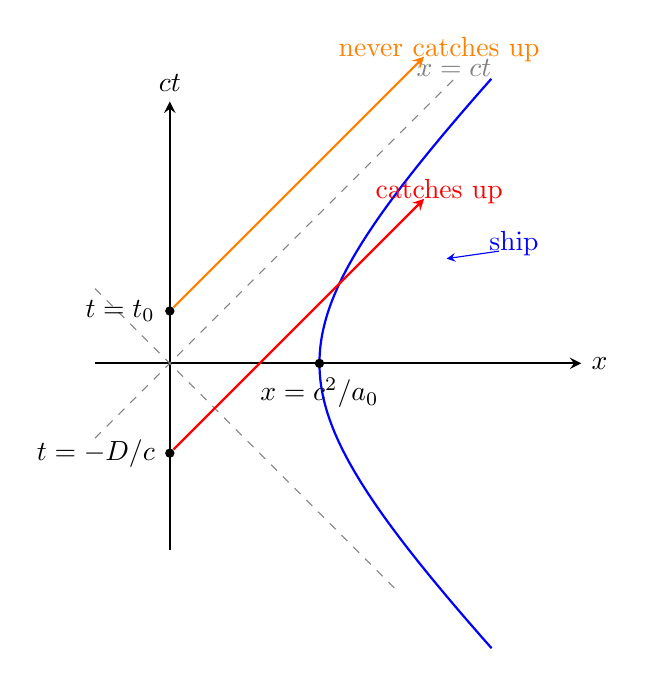
\begin{tikzpicture}[>=stealth, scale=0.95]
  % axes
  \draw[->, thick] (-1.0,0) -- (5.5,0) node[right] {$x$};
  \draw[->, thick] (0,-2.5) -- (0,3.5) node[above] {$ct$};
  % light cone (asymptote)
  \draw[dashed,gray] (-1.0,-1.0) -- (3.8,3.8);
  \node[gray] at (3.8,3.95) {$x=ct$};
  \draw[dashed,gray] (-1.0,1.0) -- (3.0,-3.0);
  % ship hyperbola: x = R cosh t, ct = R sinh t, R=2
  \draw[thick,blue,domain=-1.4:1.4,samples=80,smooth,variable=\t]
    plot ({2*cosh(\t)},{2*sinh(\t)});
  \node[blue] at (4.6,1.6) {ship};
  \draw[blue,->,thin] (4.4,1.5) -- (3.7,1.4);
  % closest approach point
  \node[circle,fill,inner sep=1.2pt,label=below:{$x=c^2/a_0$}] at (2,0) {};
  % photon from (-D/c, 0): emits at (0,-1.2), reaches ship
  \node[circle,fill,inner sep=1.2pt,label=left:{$t=-D/c$}] (P1) at (0,-1.2) {};
  \draw[->,thick,red] (P1) -- (3.4,2.2);
  \node[red] at (3.6,2.3) {catches up};
  % photon from (0, t_0>0)
  \node[circle,fill,inner sep=1.2pt,label=left:{$t=t_0$}] (P2) at (0,0.7) {};
  \draw[->,thick,orange] (P2) -- (3.4,4.1);
  \node[orange] at (3.6,4.2) {never catches up};
\end{tikzpicture}
\end{center}
The orange ray runs forever parallel to the ship's late-time asymptote $x=ct$; the locus $x=ct$ is the Rindler horizon.

\end{document}
